%% % $Id: import.tex 10719 2010-03-26 16:43:13Z berndk $
%% % Local Variables:
%% % ispell-check-comments: nil
%% % Local IspellDict: american
%% % End:
%% % --------------------------------------------------------
%% % User documentation
%% % copyright by BREDEX GmbH 2005
%% % --------------------------------------------------------
%% % this command can be inserted multiple times
%% \gdhelpid{}
%% % 
%% \begin{bxdescription}
%% \end{bxdescription}
%% %
%% \begin{bxsteps}
%% % use the \item command for single steps
%% \end{bxsteps}
%% % change <FILE> to the same filename you are editing
%% \bxinput{Links/<FILE>}
%% %
%% % other usefull commands are
%% %   \bxhint{}        to create a hint
%% %   \bxwarn{}        to describe a warning

\index{Project!Import}
\index{Import!Project}
\index{Import!Test Case}
\index{Test Case!Import}
You can import whole \gdprojects{} \bxpref{ImportProject} or the \gdcases{} \bxpref{ImportTestCases} from a specific \gdproject{} into the current \gdproject{}. 

\subsection{Importing whole \gdprojects{}}
\label{ImportProject}

\begin{enumerate} 
\item To import whole \gdprojects{} from a \gdproject{}, select:\\
 \bxmenu{Project}{Import}{}. 
\item In the dialog which appears (\bxfigref{Import}), enter or browse to the \gdproject{} you want to import. 

\item If you have entered the path to a \gdproject{}, click \bxcaption{Add} to add it to the list of \gdprojects{} to be imported. 

\bxtipp{Note that the \bxcaption{Add} button will only be activated if the path you have entered is correct.} 

If you add multiple \gdprojects{} to be imported, you can change the order they are imported in using the arrows next to the list of \gdprojects{}. You can also remove a \gdproject{} from the list of \gdprojects{} to be imported. 

\bxtipp{If you are importing \gdprojects{} that are dependent on other \gdprojects{} (i.e. they reuse other \gdprojects{}), import the supporting \gdprojects{} first.}
\item If you only want to import one whole \gdproject{}, you can select the option to open the \gdproject{} once it has been imported. 

\item When you have finished your selection, click \bxcaption{OK}. The \gdprojects{} you selected will be imported in the order specified. 
\end{enumerate}

\subsection{Importing \gdcases{} from \gdprojects{}}
\label{ImportTestCases}
\begin{enumerate}
\item To import the \gdcases{} from one or more \gdprojects{}, select:\\
 \bxmenu{Project}{Import}{}. 
\item In the dialog which appears (\bxfigref{Import}), enter or browse to the \gdprojects{} whose \gdcases{} you want to import. 

\bxtipp{You can only import \gdcases{} from \gdprojects{} whose toolkit is supported by the current \gdproject{}.}

\begin{figure} [htbp]
\begin{center}
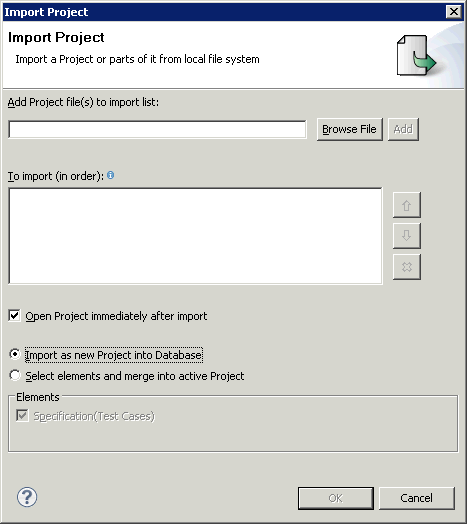
\includegraphics{Tasks/Projects/PS/Import}
\caption{Import Dialog}
\label{Import}
\end{center}
\end{figure}

\item If you have entered the path to a \gdproject{}, click \bxcaption{Add} to add it to the list of \gdprojects{}.  

\bxtipp{Note that the \bxcaption{Add} button will only be activated if the path you have entered is correct.} 

If you add multiple \gdprojects{}, you can change the order in which their \gdcases{} are imported in using the arrows next to the list of \gdprojects{}. You can also remove a \gdproject{} from the list of \gdprojects{}. 

\bxtipp{If you are importing \gdprojects{} whose \gdcases{} are dependent on other \gdprojects{} (i.e. they reuse other \gdprojects{}), import the supporting \gdprojects{} first.}

\item Select the option to import partial \gdprojects{}. 
\item When you have finished your selection, click \bxcaption{OK}. The \gdcases{} from \gdprojects{} you selected will be imported in the order specified. 
\item The \gdcases{} are imported directly into the currently opened \gdproject{}. They can be found in the category \bxname{ImportedTCs}. 
\end{enumerate}

\bxtipp{Importing \gdcases{} in this way is different from importing reused \gdcases{} from a reusable \gdproject{} \bxpref{reuseproject}. Reusable \gdcases{} are read-only, and are affected by any changes made in their original \gdproject{}. Imported \gdcases{} can be modified normally, and are not affected by any changes in their original \gdproject{}. They are essentially copies. If you want to work with \gdproject{} libraries, we recommend reusing \gdprojects{} instead of importing their \gdcases{}.} 


